\documentclass[lettersize,journal]{IEEEtran}
\usepackage{amsmath,amsfonts}
\usepackage{algorithmic}
\usepackage{algorithm}
\usepackage{array}
\usepackage[caption=false,font=normalsize,labelfont=sf,textfont=sf]{subfig}
\usepackage{textcomp}
\usepackage{stfloats}
\usepackage{url}
\usepackage{verbatim}
\usepackage{graphicx}
\usepackage{cite}
\usepackage{color}
\hyphenation{op-tical net-works semi-conduc-tor IEEE-Xplore}
% updated with editorial comments 8/9/2021

\begin{document}
\title{Industrial Stack Emissions Monitoring: Enhancing Pollution Assessment with Multirotor Drone Technology}
\author{
Mojtaba Bahrami
and
Afshin Banazadeh

\thanks{Manuscript received Month DD, YYYY; revised Month DD, YYYY.}
\thanks{Authors are with Department of Aerospace Engineering, Sharif University of Technology, Tehran, Iran}
}

% The paper headers
\markboth{IEEE Transactions on Geoscience and Remote Sensing,~Vol.~xx, No.~x, monthx~yearx}
{Shell \MakeLowercase{\textit{et al.}}: A Sample Article Using IEEEtran.cls for IEEE Journals}

% \IEEEpubid{0000--0000/00\$00.00~\copyright~2021 IEEE}
% Remember, if you use this you must call \IEEEpubidadjcol in the second
% column for its text to clear the IEEEpubid mark.

\maketitle

\begin{abstract}
This research focuses on the conceptual design of a novel stack emissions monitoring aerial platform, addressing the critical issue of monitoring industrial stacks to control air pollution. The inherent risks associated with monitoring tall stacks, particularly in refineries, pose threats to human lives and health. By employing an aerial robotic system, these risks are eliminated while simultaneously reducing time and operational costs. Through rigorous demand and mission analysis, the design process is structured into five stages: 1. Selection of an avian-inspired manipulator and sampling probe, 2. Configuration layout, 3. Selection of an appropriate monitoring sensor, 4. Iterative weight estimation and propulsion selection, and 5. Identification of subsystems and key components. To optimize the manipulator's installation, an optimization process is employed. Design decisions are guided by quantified criteria, ensuring a systematic and objective approach. The presented novel design sketch exemplifies the potential of the proposed concept, emphasizing the importance of adopting a systematic design view in effectively addressing the critical issue of stack emissions monitoring. \textcolor{red}{\emph{(This is the previous abstract, so it's better to revise and finalize it later).}}
\end{abstract}

\begin{IEEEkeywords}
Air pollution monitoring, Aerial emissions monitoring, Manipulator design, Multirotor conceptual design, Drone remote sensing, Aerial inspection.
\textcolor{red}{\emph{(Needs to be revised and finalized).}}
\end{IEEEkeywords}

\section{Introduction} \label{sec.intro}
\IEEEPARstart{A}{IR} pollution has become a pressing global issue, exacerbated by rapid urbanization and industrialization ~\cite{barbera2010hyperbolic}. This phenomenon has led to significant public health concerns, including respiratory and cardiovascular diseases, and has been linked to increased mortality rates ~\cite{zarrar2023drive}. According to the World Health Organization, over 99\% of the global population breathes air that exceeds guideline limits ~\cite{WHO-poluted99}, making air pollution one of the grand health challenges of our time ~\cite{world2016ambient}.

Monitoring emissions from industrial stacks is a critical component of environmental protection. Traditional methods rely heavily on manual inspections, where operators physically ascend to the stack's inspection flange, insert a probe, and collect data ~\cite{testo350application}. This approach is not only labor-intensive and time-consuming but also poses substantial risks to human operators, particularly in hazardous environments such as refineries and chemical plants. Data from the U.S. Department of Labor indicates that, between 2018 and 2022, over 800 workplace fatalities annually were attributed to falls ~\cite{Injuries2022}, highlighting the inherent dangers of such tasks.

The use of unmanned aerial vehicles (UAVs), for inspection and monitoring has advanced significantly in recent years ~\cite{qiu2017low}. UAVs equipped with low-cost air quality sensors offer a scalable and high-resolution solution for air quality monitoring, enabling rapid coverage of large areas ~\cite{motlagh2023unmanned}. For instance, UAVs have been employed to create pollution maps by collecting and transmitting data to a base station ~\cite{alvear2017using}, and to estimate air quality indices (AQI) using aerial imagery ~\cite{gao2020aq360}. Dow’s Manufacturing 4.0 initiative has successfully utilized UAVs for remote inspections, resulting in substantial cost savings and a reduction in confined space entries, thereby enhancing safety and productivity ~\cite{kas2020using}.

UAVs have also been employed to localize emission sources. For example, a UAV system model has been proposed for detecting air pollution sources ~\cite{le2022efficient}, and a path-planning framework has been developed to schedule UAV flight paths for identifying excessive emission stacks in industrial areas ~\cite{wang2024efficient}. These applications demonstrate the potential for increased inspection frequency, leading to quicker identification and repair of emitting facilities, thereby reducing overall emissions ~\cite{rashid2020optimized}.

Despite the advancements in environmental monitoring and source localization, there remains a critical gap in the accurate monitoring of stack emissions using UAVs. This gap necessitates the continued exposure of inspectors to hazardous conditions. In this article, we address this issue by designing an aerial platform capable of autonomously carrying an inspection device to the stack's inspection flange, inserting the probe, and collecting data fast, efficiently and safely.

\textcolor{red}{\emph{(Remember to write a summary here.)}} The organization of this article is listed as follows ...

\section{Problem Description}
Aerial monitoring of industrial stack emissions is a critical task that requires a comprehensive system. This system must encompass various components, including an aerial vehicle, telecommunication equipment, maintenance protocols, operational guidelines, control and navigation systems, safety measures, and more. This research focuses exclusively on the design of the aerial vehicle.

The mission profile is illustrated in figure \ref{fig.mission}. The aerial vehicle is initially brought near the industrial zone by the pilot/operator. It then takes off, climbs to a safe altitude, and proceeds to the inspection location. While hovering near the stack, it inserts the sampling probe, collects data, and retracts the probe. Following inspection, the drone returns, descends, and lands. The design must accommodate the drone's mission and its payload, including the inspection device, sampling probe, and a robotic arm for probe manipulation.

\begin{figure}[!t]
\centering
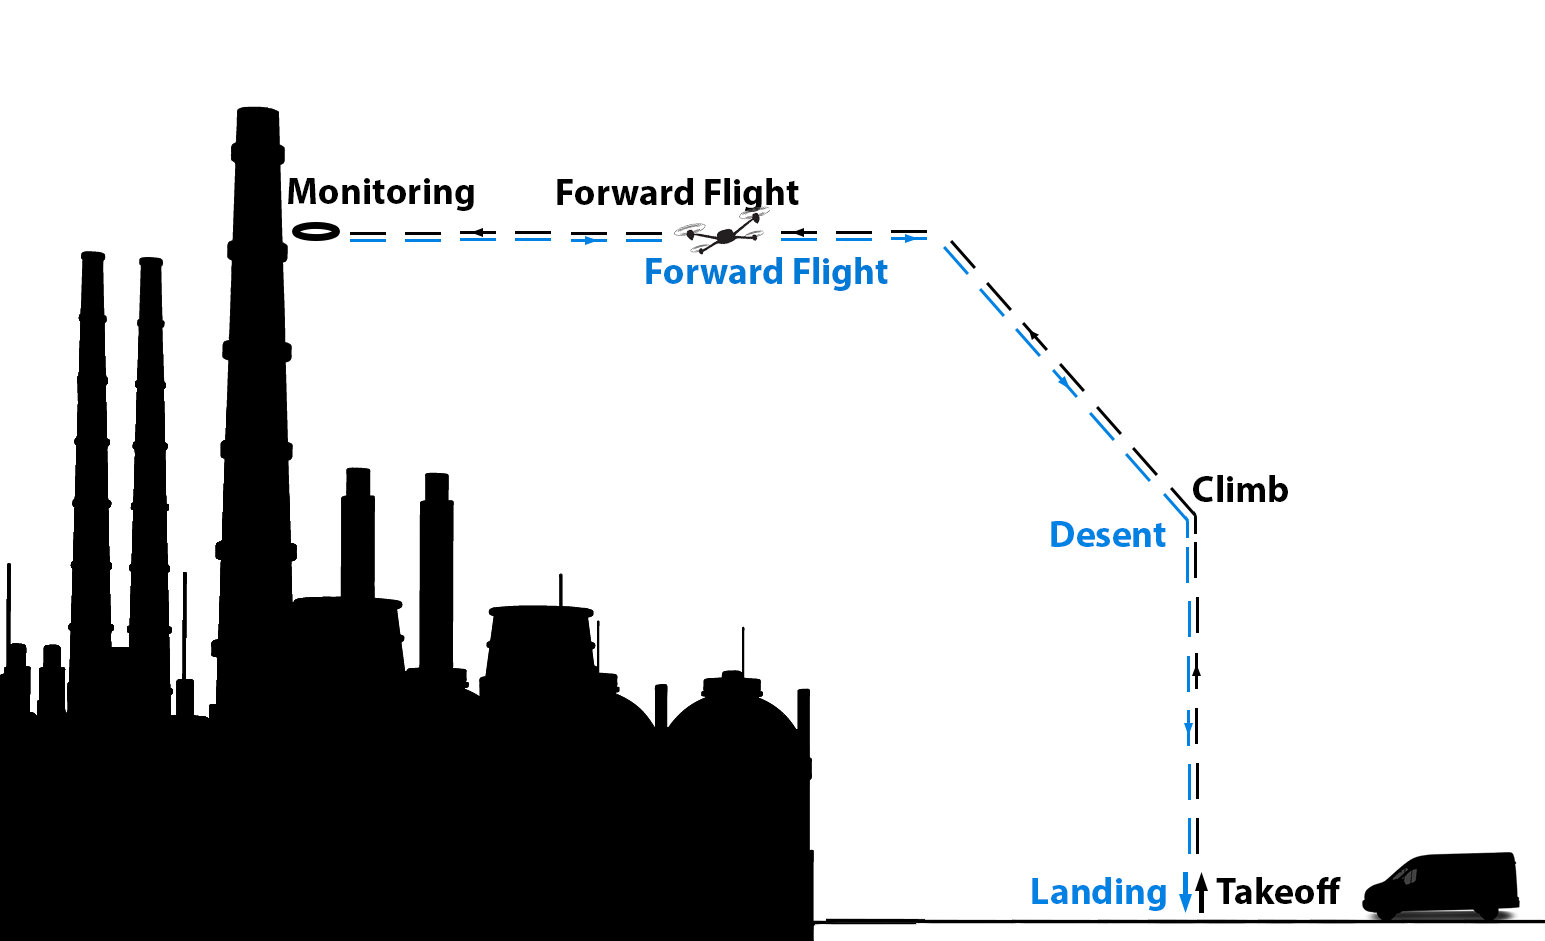
\includegraphics[width=3.45in]{./Pictures/MissionDiagram}
\caption{Aerial emissions monitoring of industrial stacks mission profile}
\label{fig.mission}
\end{figure}

Given the high probability of collision when operating near the chimney, risk mitigation measures are essential. Operating within an industrial area adds further complications, as a crash could result in significant damage. Therefore, the drone must be designed to minimize the risk of failure. One common failure in aerial systems is engine or motor malfunction. Consequently, the aerial vehicle must be capable of operating safely even in the event of a single motor failure. To ensure a safe margin with obstacles, particularly the stack, the drone must be equipped with collision avoidance sensors.

In summary, the design objectives for the aerial platform include:
\begin{enumerate}
\item Capability of completing the mission profile depicted in figure \ref{fig.mission}
\item Capability to carry the monitoring device.
\item Equipped with an autonomous robotic arm for precise probe manipulation.
\item Ensure safe operation in close proximity to chimneys and within industrial environments.
\item Ability to operate safely even in the event of a single motor failure.
\end{enumerate}


\section{Design Constraints}
\subsection{Mission Profile Requirements}
\subsection{Regulations and Safety Considerations}
\subsection{Standard Flange}
Currently, industrial stacks are equipped with inspection flanges featuring covers to prevent leakage and protect against infiltration. These covers, secured with bolts and nuts, are designed for human operators but require a heavy manipulator for aerial platforms. Figure \ref{fig.typflange} illustrates a typical flange.

\begin{figure}[!t]
\centering
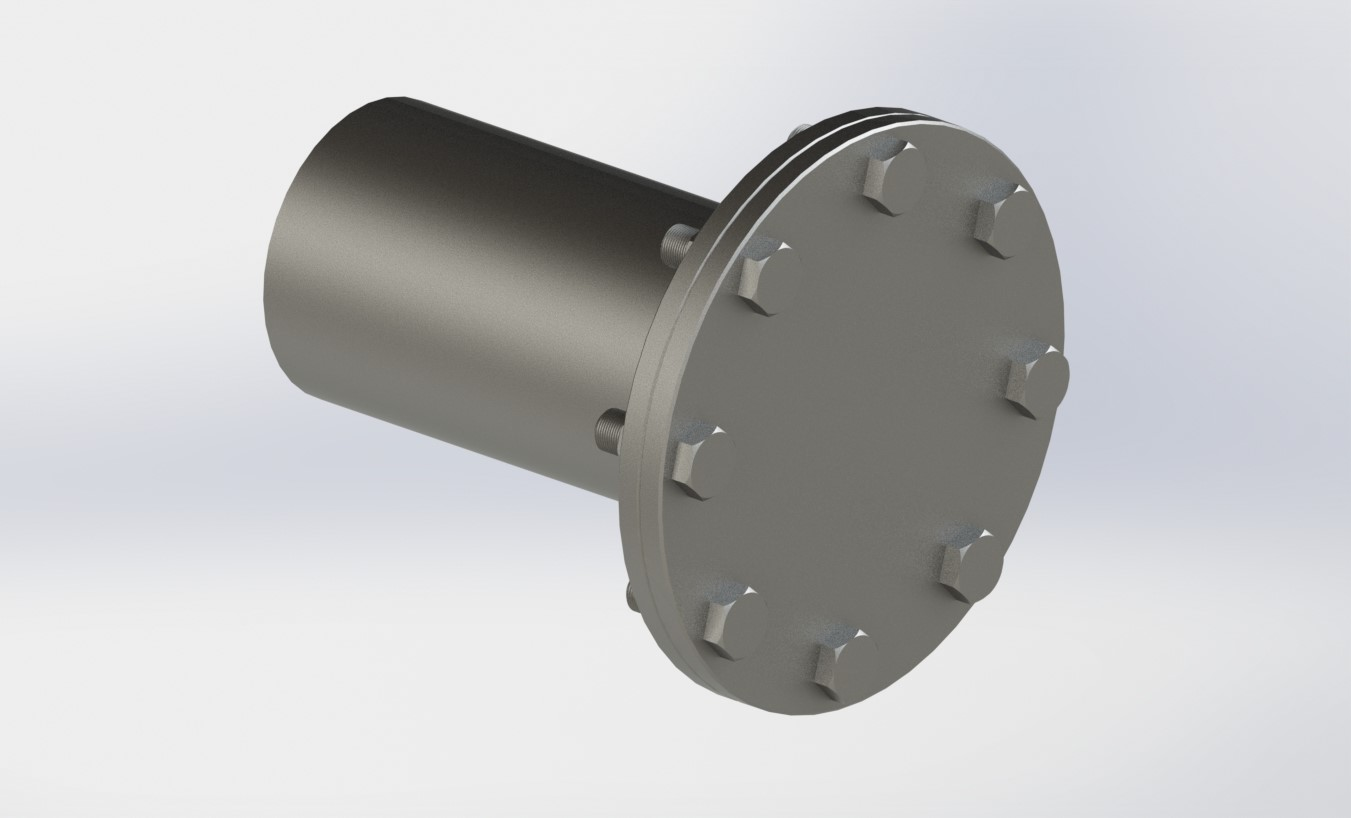
\includegraphics[width=2.45in]{./Pictures/TypicalFlangeAndCover}
\caption{A typical monitoring flange CAD model}
\label{fig.typflange}
\end{figure}

A solution is to standardize flange covers by replacing current designs with ones suitable for aerial stack monitoring. These covers/caps should:
\begin{enumerate}
\item Eliminate the use of bolts and nuts, removing the need for heavy robotic arms.
\item Be effortlessly easy to open (for example, using a spring hinge mechanism for opening and closing, while accounting for thermal expansion).
\item Prevent chimney smoke from escaping.
\item Have a sufficiently large diameter to allow easy probe entry and exit.
\end{enumerate}

Additionally, these flanges are better to be easily identifiable by a camera. Figure \ref{fig.stdflange} presents a typical example. This example demonstrates how common covers can be modified to become suitable for use with an aerial manipulator.

\begin{figure}[!t]
\centering
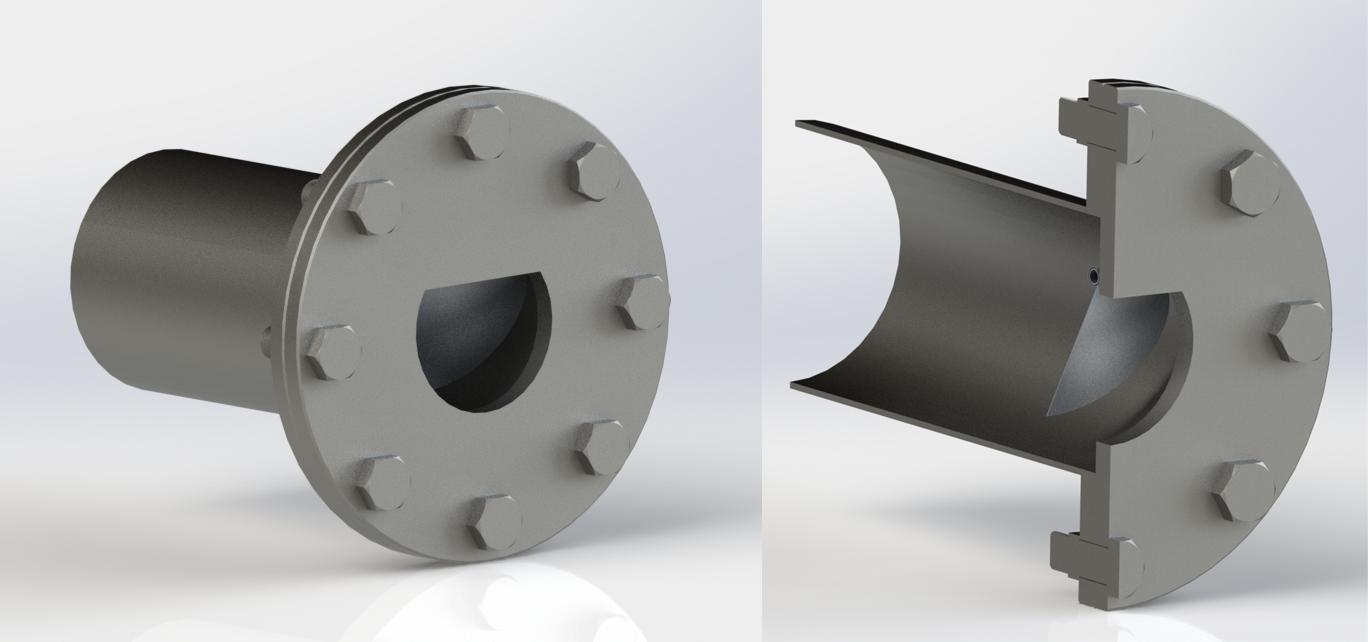
\includegraphics[width=2.45in]{./Pictures/StandardFlangeAndCoverDual}
\caption{A standardized monitoring flange CAD model}
\label{fig.stdflange}
\end{figure}

\section{Design Required Data}
In this section, we will navigate through the available data required for the design process. All of this data is gathered in \cite{githubrepo2025}..

\subsection{Emission Monitoring Sensors}
in Table~\ref{tab1}.
\begin{table}
\begin{center}
\caption{Specifications of Emission Monitoring Devices}
\label{tab1}
\begin{tabular}{| c | c | c |}
\hline
Device & Mass (g) & Dimension (mm)\\
\hline
Testo 350\cite{testo350specs} & 4800 & $330 \times 128 \times 438$ \\
\hline
MRU NOVA Plus\cite{MRUNovaPluseSpecs} & 7400 & $470 \times 314 \times 235$ \\
\hline
MRU VARIO Luxx\cite{MRUVARIOLuxx} & 7500 & $430 \times 290 \times 150$ \\
\hline
AMETEK Land Lancom 4\cite{AMETEKLandLancom4} & 6000 & $453 \times 120 \times 245$ \\
\hline
\end{tabular}
\end{center}
\end{table}

\subsection{Similar Multi-rotors (with respect to payload weight)}
\subsection{Propulsion Systems}
\subsection{Batteries}

\section{Aerial Platform Architecture}
\subsection{Emission Monitoring Sensor}
\subsection{Multi-rotor Configuration}


\subsection{Manipulator Design}
Once the flying vehicle is positioned in front of the flange and is ready for sampling, the probe should be inserted into the chimney. After completing the sampling and monitoring the chimney gas, the probe should be removed. A manipulator is required to accomplish this task. This manipulator, with the mechanism described in this section, will carry out this part of the mission. But how can we determine if this manipulator mechanism will be effective? In a situation where there is no error in the position of the flying vehicle, a linear motion is sufficient for the probe to enter and exit. However, if there is a positional error, the manipulator's movement mechanism needs to compensate for this error. Therefore, this manipulator needs to be capable of moving in three directions. The mechanisms in Figure \ref{fig.3d_mechanisms} have the ability to cover a limited three-dimensional space.

\begin{figure}[!t]
\centering
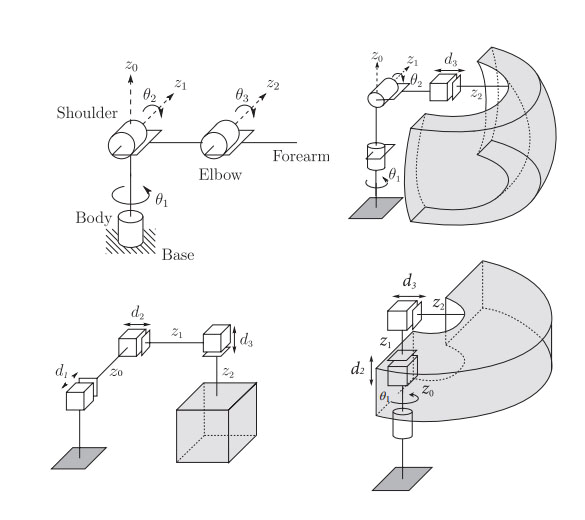
\includegraphics[width=2.45in]{./Pictures/3D_Mechanisms}
\caption{Common mechanisms with a three-dimensional workspace ~\cite{spong2020robot}}
\label{fig.3d_mechanisms}
\end{figure}

Now consider a situation where the flying vehicle also has a status error. In such a situation, the robotic arm must also be able to correct these errors. In other words, the robotic arm must be able to control the probe's position independently of the flying vehicle. A wrist mechanism is used for this task. This mechanism is shown in Figure \ref{fig.wrist_mechanism}.

\begin{figure}[!t]
\centering
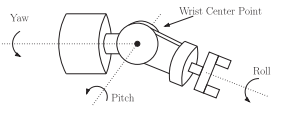
\includegraphics[width=2.45in]{./Pictures/Wrist_Mechanim}
\caption{Wrist mechanism ~\cite{spong2020robot}}
\label{fig.wrist_mechanism}
\end{figure}

In addition to these factors, the lightness of the robotic arm, and the ability to withstand the weight of the probe and the force of the flange door are also requirements that must be considered. Since the rotational joints have a higher torque tolerance than the linear ones and also weigh less, the mechanism shown in Figure \ref{fig.probe_mechanism} can be considered as the overall mechanism of the probe's robotic arm.

\begin{figure}[!t]
\centering
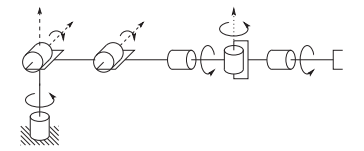
\includegraphics[width=2.45in]{./Pictures/Probe_Mechanim}
\caption{Probe manipulator mechanism ~\cite{spong2020robot}}
\label{fig.probe_mechanism}
\end{figure}

\subsection{Weight Estimation and Propulsion System Selection}

\begin{multline}\label{eq:W.Takeoff}
\text{$W_{Takeoff} = W_{Frame} + W_{Payload} + $}\\
\text{$W_{Propulsion\ System} + W_{Equipments}$}
\end{multline}
\begin{multline}\label{eq:W.Payload}
\text{$W_{Payload} = $}\\
\text{$W_{Inspection\ Device} + W_{Probe} +W_{Manipulatior}$}
\end{multline}
\begin{multline}\label{eq:W.PropulsionSystem}
\text{$W_{Propulsion\ System} = W_{Motors} + W_{Props} + W_{ESCs}$}
\end{multline}
\begin{multline}\label{eq:W.Equipments}
\text{$W_{Equipments} = W_{Batteries} + W_{On-Board\ Camera} + $}\\
\text{$W_{Range\ Finder} + W_{On-Board\ Computer} + $}\\
\text{$ W_{Flight\ Controllers} + W_{Other\ Electronic\ Devices}$}
\end{multline}

\begin{algorithm}[H]
\caption{Weight Estimation and Propulsion System Selectio Algorithm}\label{alg:WeightEst}
\begin{algorithmic}
\STATE
\STATE
\end{algorithmic}
\end{algorithm}

\subsection{Other Main Equipments}
\subsubsection{On-Board Computer}
\subsubsection{Multiple (Redundant) Autopilots}
\subsubsection{Range Finder}
\subsubsection{On-Board Camera}
\subsubsection{Data Transceivers}

\section{Implementation Challenges}

\section{Conclusion}

\section*{Acknowledgments}

%{\appendix}
%{\appendices}


\bibliography{References}{}
\bibliographystyle{IEEEtran}

\newpage

\section{Biography Section}

\vfill

\end{document} 